\documentclass[12pt, a4paper]{article}

\usepackage{amsmath, amssymb, amsthm}
\usepackage[margin=0.5in]{geometry}
\usepackage{algorithm,algpseudocode}
\usepackage{bm}
\usepackage{wrapfig}
\usepackage{subcaption}
\usepackage{mathtools}
\usepackage{chngcntr}
\usepackage{framed}
\usepackage{xcolor}
\usepackage{setspace}
\usepackage{biblatex}
\usepackage{minted}
\usepackage{physics}
\usepackage{mathdots}
\usepackage{yhmath}
\usepackage{cancel}
\usepackage{color}
\usepackage{siunitx}
\usepackage{array}
\usepackage{multirow}
\usepackage{amssymb}
\usepackage{gensymb}
\usepackage{tabularx}
\usepackage{extarrows}
\usepackage{booktabs}
\usepackage{placeins}
\usepackage{graphicx}
\graphicspath{ {./images/} }
\usepackage{tikz}
\usetikzlibrary{arrows}
\usetikzlibrary{shapes}
\usetikzlibrary{fadings}
\usetikzlibrary{patterns}
\usetikzlibrary{shadows.blur}

\counterwithin{figure}{section}

% \makeatletter
% \def\@seccntformat#1{
%   \expandafter\ifx\csname c@#1\endcsname\c@section\else
%   \csname the#1\endcsname\quad
%   \fi}
% \makeatother

\addbibresource{citation.bib}

\renewcommand\qedsymbol{QED}
\renewcommand{\familydefault}{\sfdefault}

\newcommand*\circled[1]{\tikz[baseline=(char.base)]{
            \node[shape=circle,draw,inner sep=2pt] (char) {#1};}}

\newtheorem{theorem}{Theorem}[section]
\newtheorem{lemma}{Lemma}[section]

\newcommand{\code}[1]{\mintinline{cpp}|#1|}

\begin{document}
    \begin{minipage}[]{\textwidth}
        \setstretch{1.25}
        \centering{
            \Huge Project Report \par
            \Large \textcolor{darkgray}{Introduction to Algorithm Engineering} \par
            \large \textcolor{darkgray}{Bharat Sahlot | Kyrylo Shyvam Kumar} \par
        }
        \setstretch{1.0}
    \end{minipage}

    \section{Introduction}
    
    The paper\cite{paper} presents a data structure and relevant algorithms for fast t-distance queries. We implemented the algorithms for connected undirected weighted graphs represented using Adjacency List.

    \section{Data Structure}

    The data structure presented is called \emph{Oracle}. It requires a pre-processing step. The pre-processing step does most of the work, therefore queries are really fast.

    The data structures takes as input a connected undirected weighted graph $G$ and an integer $K$.

    \subsection{Pre process Algorithm}

    According to the paper this step takes time $O(kmn^{\frac{1}{k}})$. The actual time complexity depends on the shortest path algorithm used. In our case we went with djikstra, therefore we have a slightly worse time complexity.

    The algorithm selects vertices randomly with a probability of $\frac{1}{k}$. We used \code{std::bernoulli_distribution} for this. We used STL data structures like \code{std::vector}, \code{std::priority_queue} and \code{std::unordered_map} heavily. We also use \code{boost::heap::fibonacci_heap} for implementation using Fibonacci Heap.

    \subsection{Query Algorithm}

    This is a simple algorithm. It takes two vertices as input and returns the k-spanner distance between them.

    \section{Performance}

    We have two implementations of the algorithm (one using \code{std::priority_queue} and other using \\
    \code{boost::heap::fibonacci_heap}), we compare them against Floyd-Warshall and Dijkstras algorithm.

    \subsection{Random Graphs}

    We generate random connected graphs of different vertices and edges, and we obtained the following performance graph.
    To account for varying nature of random graphs, around 10 were generated for given parameters to make sure data follows appropriate distribution.
\\
    
    \subsubsection{ Varying number of edges while keeping number of vertices constant:}
    \begin{figure}[H]
    \caption*{Figure-1}
    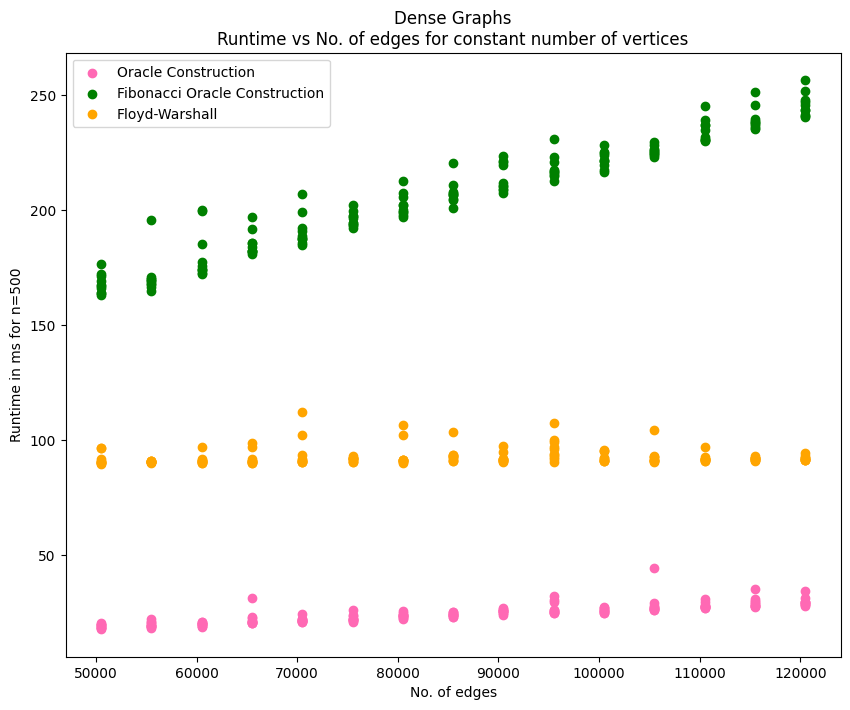
\includegraphics[scale=0.4]{./images/1}
    \centering
    \end{figure}
    In the given Figure-1, it can be noticed that Floyd-Warshall's runtime remains same and Fibonacci Heap Oracle has increasing runtime. For Normal Oracle it is also increasing, with less visibility. The increase is because of theoretical complexity of $O(kmn^{\frac{1}{k}})$.
    \begin{figure}[H]
    \caption*{Figure-2 and Figure-3}
    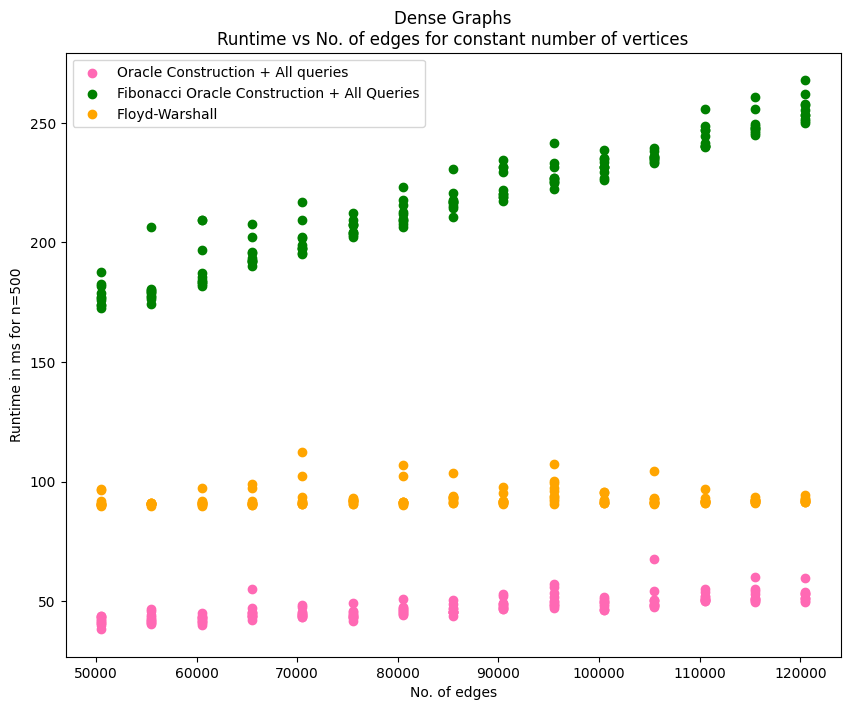
\includegraphics[scale=0.4]{./images/2}
    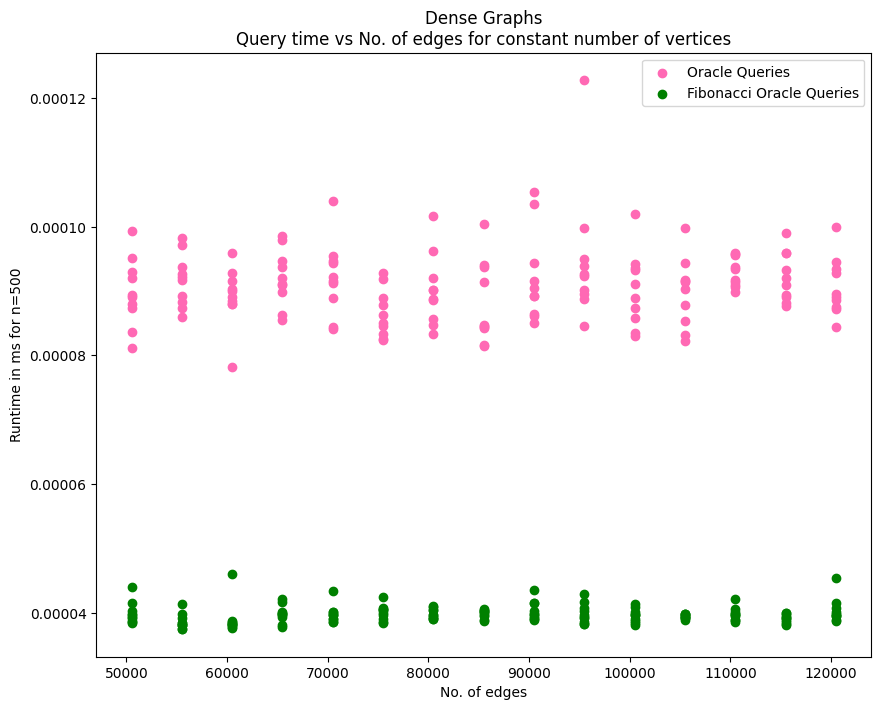
\includegraphics[scale=0.4]{./images/3}
    \end{figure} 
    The Figure-2 contains a similar as previous plot, but with accounting for querying time for all pairs of edges. The little shift of runtime of oracles can be observed.
    The next Figure compares the querying times of both Oracles. There is no increase as the number of edges increases, but the normal Oracle is a little worse due to difference in implementations.

    \begin{figure}[H]
    \caption*{Figure-3,4,5}
     
    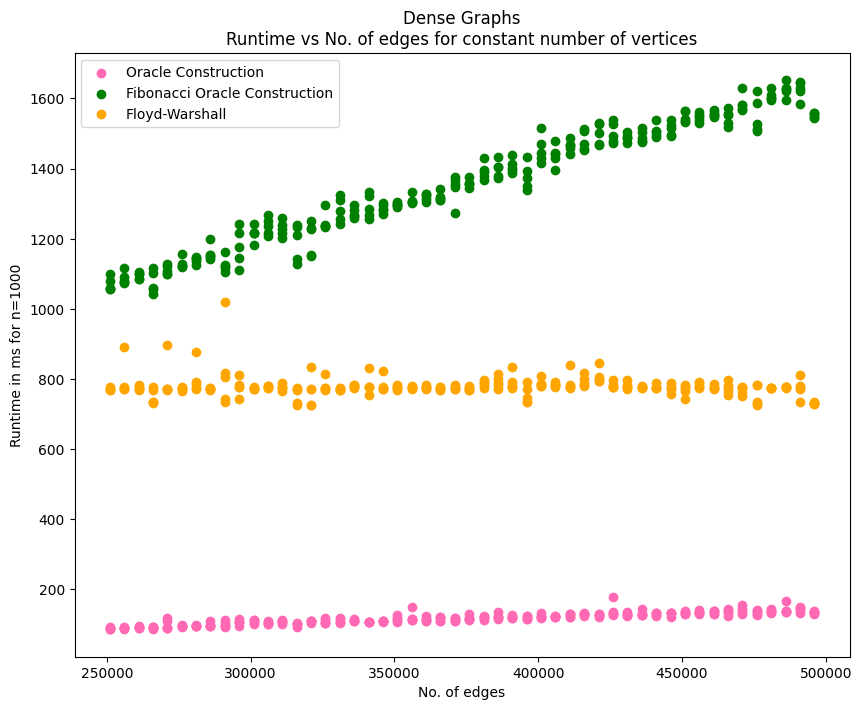
\includegraphics[scale=0.4]{./images/4}
    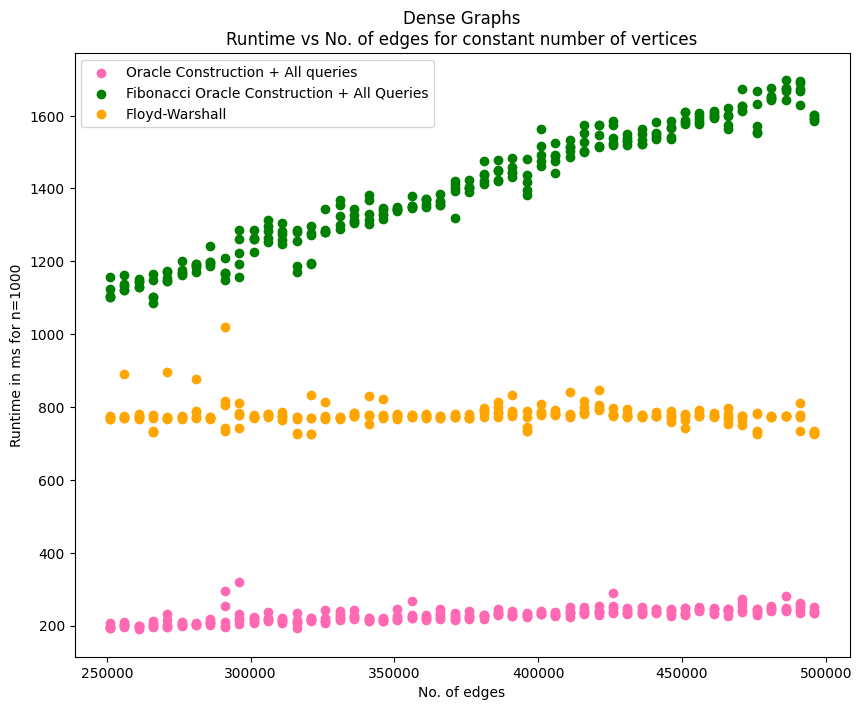
\includegraphics[scale=0.4]{./images/5}
     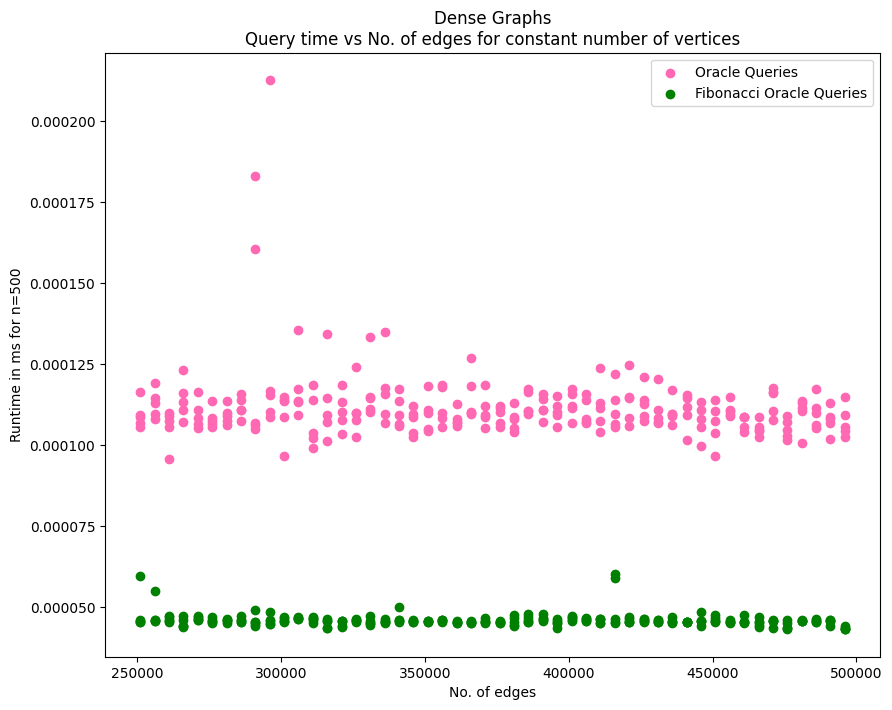
\includegraphics[scale=0.5]{./images/6}
     \centering
    \end{figure} 

    \subsubsection{Varying number of vertices while keeping number of edges constant:}
        \begin{figure}[H]
    \caption*{Figure-7}

    \centering
    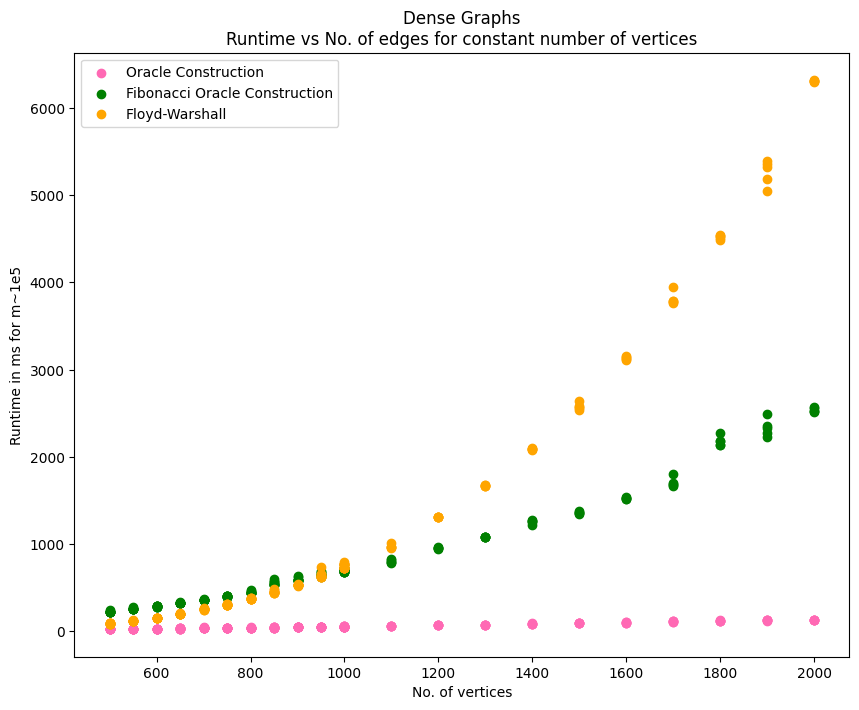
\includegraphics[scale=0.6]{./images/7}
    \end{figure} 
    
    \begin{figure}[H]
    \caption*{Figure-8,9}
    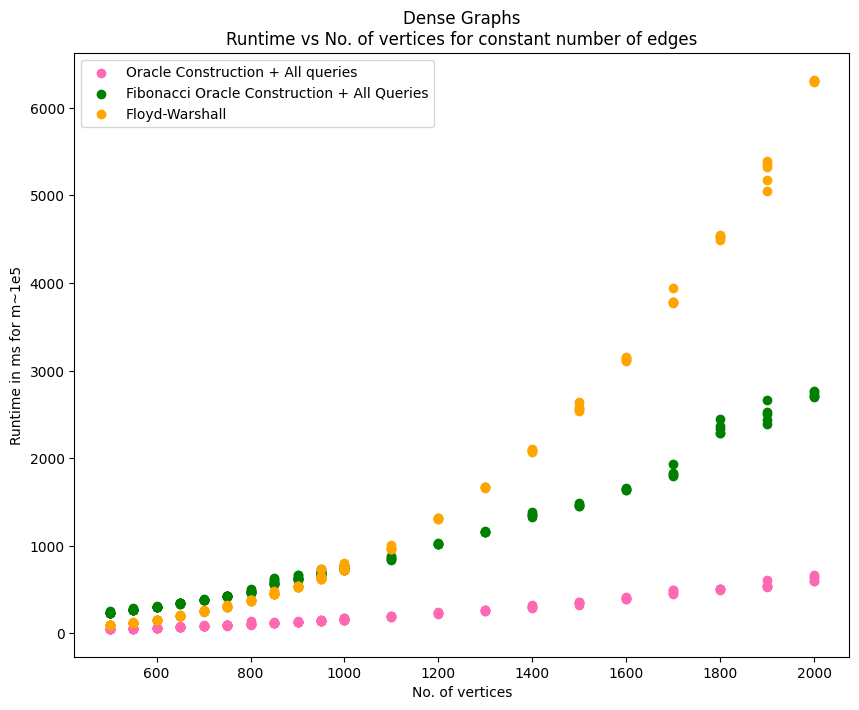
\includegraphics[scale=0.4]{./images/8}
    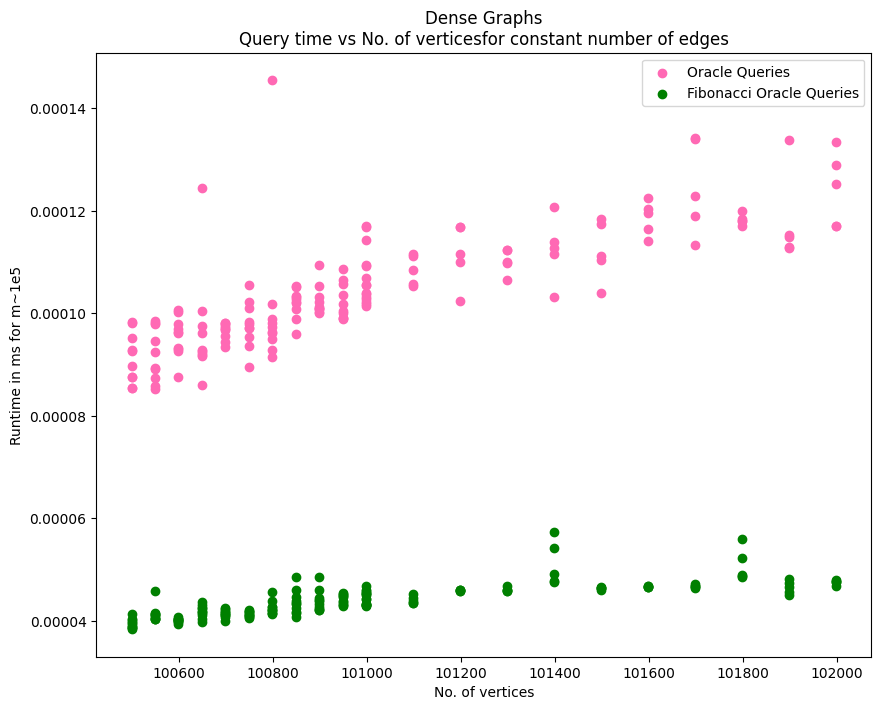
\includegraphics[scale=0.4]{./images/9}
        \centering
    \end{figure} 
 
    Here we see that runtime of Floyd-Warshall grows much faster than Oracles. The higher construction time for Oracle using Fibonacci Heap arises due to high constant factors of this data structure, but query time is unaffected and shows different trend.

    
    \subsection{Real World Graphs}
    We used 122 CAIDA-AS graphs from UoF repository. These are weighted graphs (with weights {1,2,3,4}) and we ensure that they are connected. Number of vertices stays constant at 31,379 and number of edges is around 100,000 (different for each graph). Each file contains a full
AS graph derived from a set of RouteViews BGP table snapshots.            \\
    We got these real world graphs from the \textbf{Graph} directory on the server, and we obtained the following perform-aces from them.

    \begin{figure}[H]
    \caption*{Figure-10}
    
        \centering
    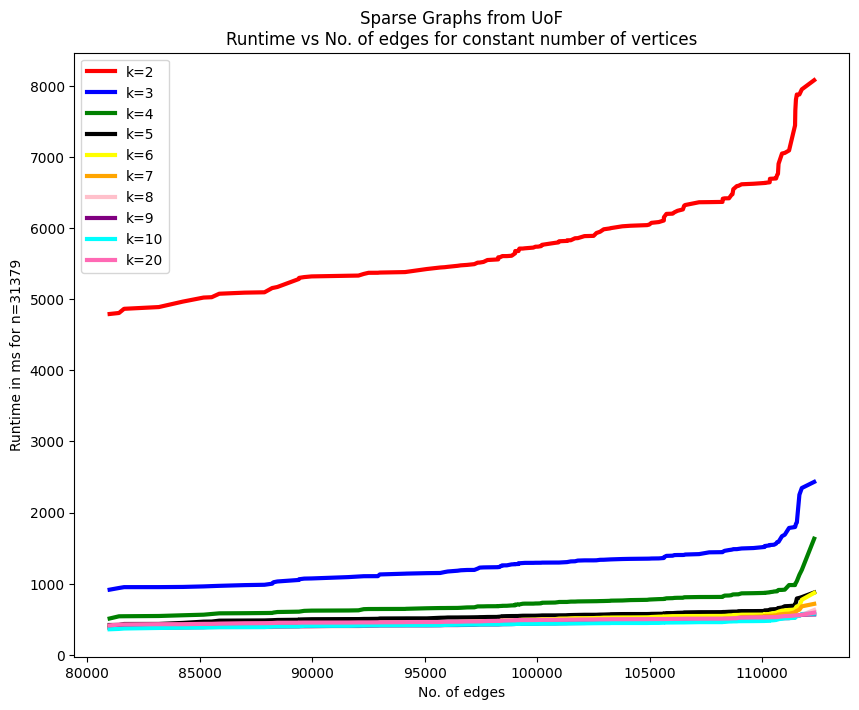
\includegraphics[scale=0.75]{./sparse/16}
    \end{figure}
    Following is a closer look on plot.
    \begin{figure}[H]
    \caption*{Figure-11,12}
    
        \centering
    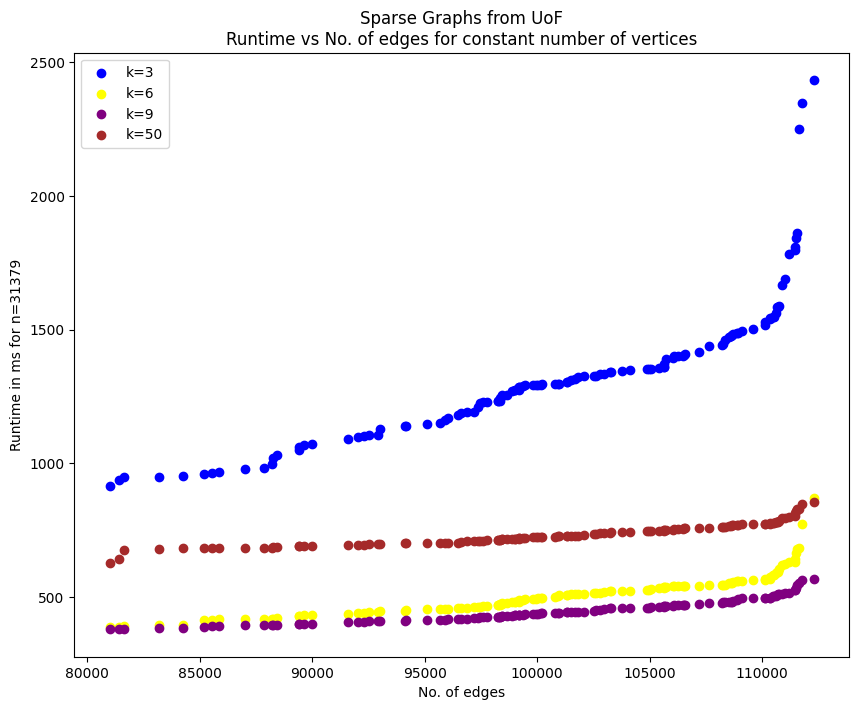
\includegraphics[scale=0.4]{./sparse/3}
     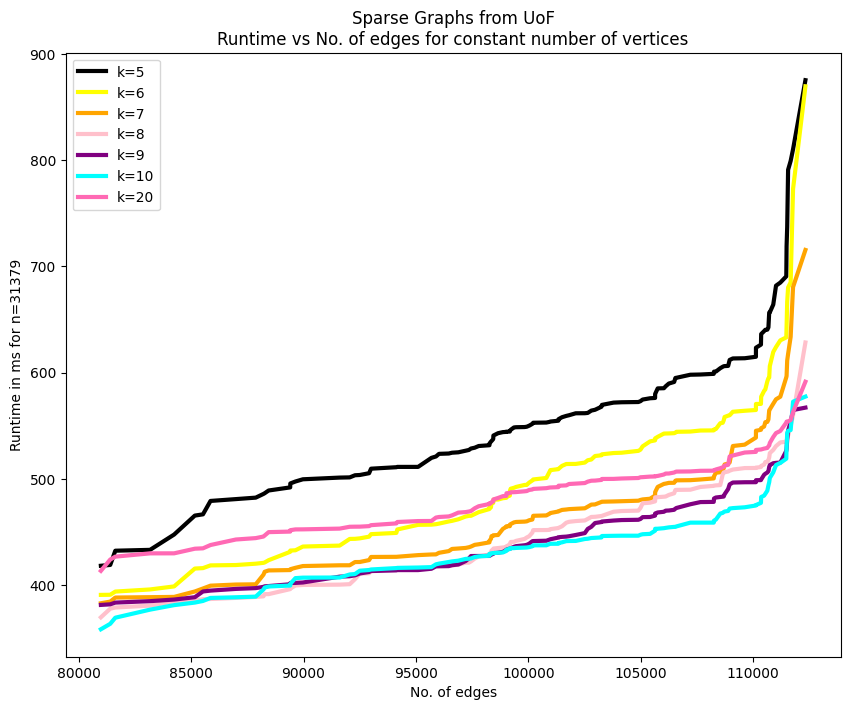
\includegraphics[scale=0.4]{./sparse/15}
    \end{figure}    

    Following represent variation of time of construction of Approximate Distance Oracle, with varying number of edges across different graphs, as well as different values of k. 
    These figures present a curious insight. The complexity of construction, decreases and then again starts to increase, with higher values of k.

    \begin{figure}[H]
    \caption*{Figure-13}
    
        \centering
    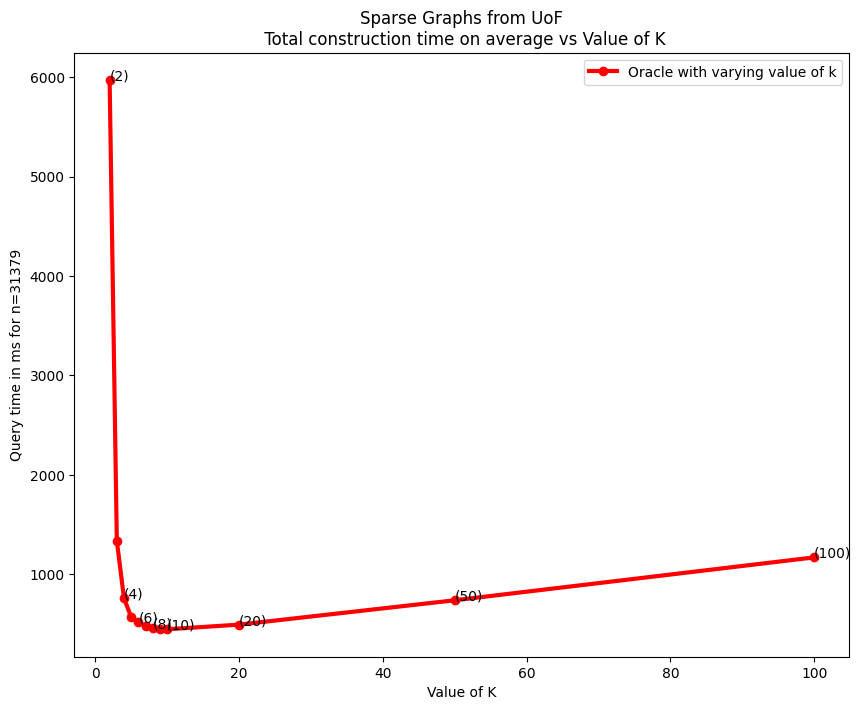
\includegraphics[scale=0.75]{./sparse/8}
    \end{figure}
    This plot is completely similar to that predicted  by $O(kmn^{\frac{1}{k}})$ complexity.

\begin{figure}[H]
    \caption*{Figure-14}    
        \centering
    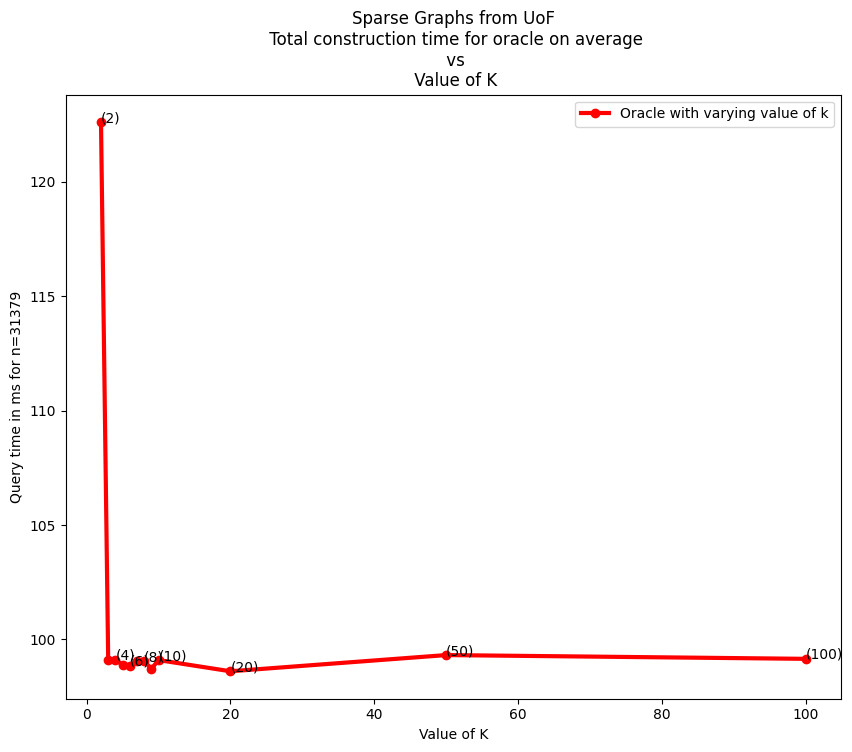
\includegraphics[scale=0.6]{./17}
    \end{figure}
    The plot shows that the change is actually minimum and not regular due to some overhead. Some increase may be noticed from 10 to 100, maybe due to the fact that its complexity is $O(k)$

\begin{figure}[H]
    \caption*{Figure-15 and 16}    
        \centering
    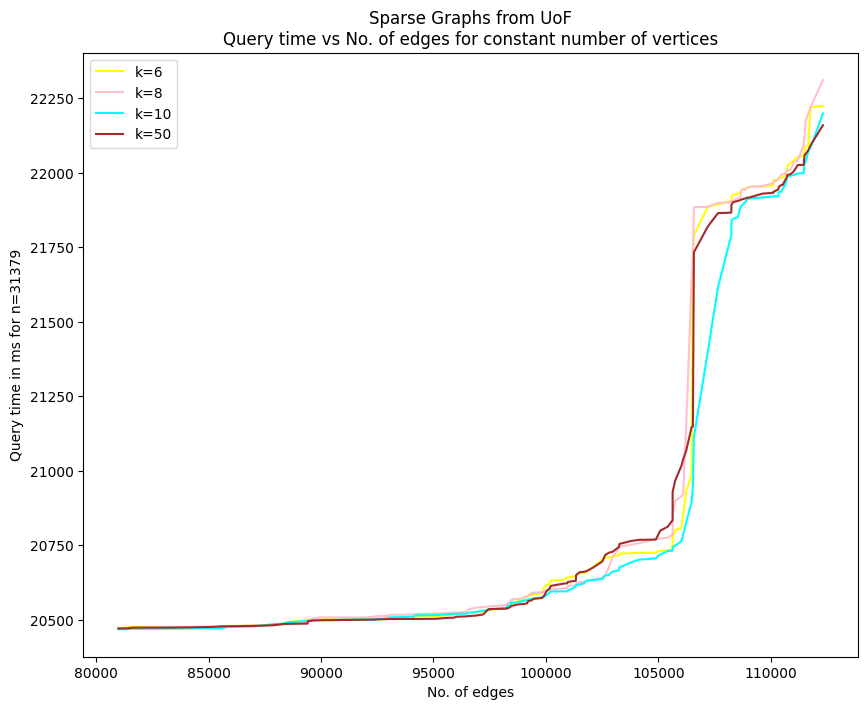
\includegraphics[scale=0.5]{./sparse/11}
        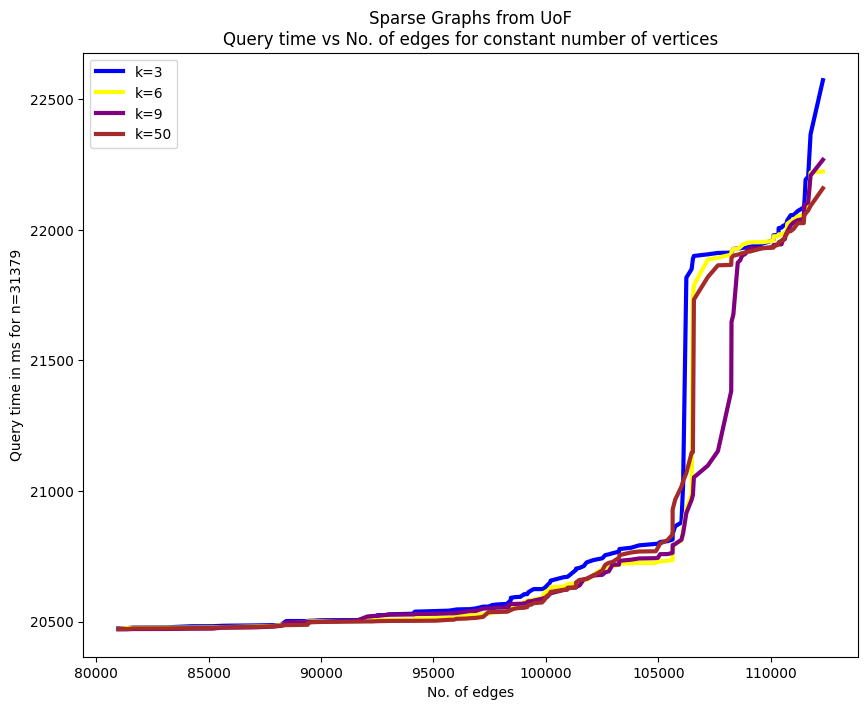
\includegraphics[scale=0.5]{./sparse/13}
    \end{figure}
These plots were showing the dependency of total query time on number of edges. Even if the actual runtime per query stays same, overall time is dependant on $O(n^2)$. The difference across all edges is not clear, but again is minimum for $k=10$, which is matching with inference coming from Figure-14.
\\\\
We also ran N-Dijkstras on the same graphs. Output can be summarized in one plot.
\begin{figure}[H]
    \caption*{Figure-14}    
        \centering
    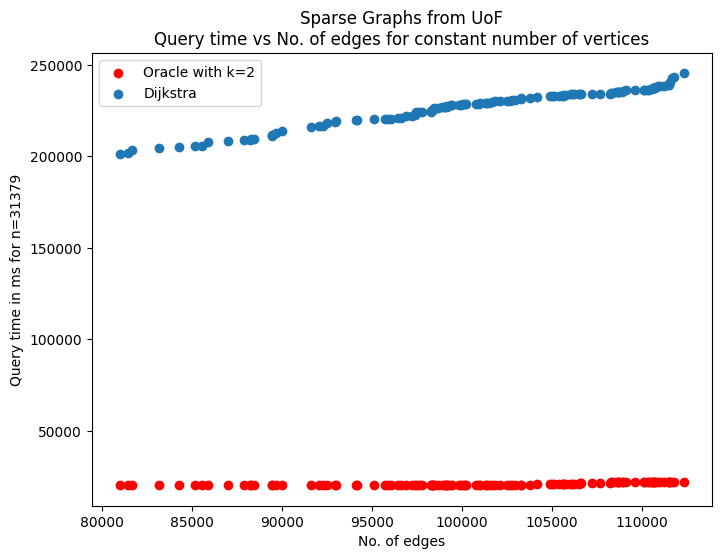
\includegraphics[scale=0.7]{./sparse/7}
    \end{figure}
    In Dijkstra, both query time as well as total query time will be function of number of vertices/edges. For Oracle total query time, will remain constant. It would vary with change in number of vertices. Each query takes constant time, and is not dependant on no. of vertices or edges. 
    \printbibliography
\end{document}
